\section{Results}
\label{sec:results}
All 360 injected fits (2 datasets $\times$ 6 ratios $\times$ 3 splits $\times$ 10 draws) and their validation-temperature-scaled sensitivity variant converged with no missing records; Table~\ref{tab:h2} reports the full curve for both.

\subsection{Gate G fails on both datasets}
\label{sec:gate-result}
$D_{\mathrm{sim}}(\rho=100)$ falls far outside the already-fitted P100 interval on both datasets, and the two failures are not the same size. On TCGA-UT, $D_{\mathrm{sim}}(100)=10.55$ points, roughly seven times the fitted point estimate of 1.20 and outside the fitted interval $[0.87, 1.53]$ by a factor of about seven at the nearer bound. On BRACS, $D_{\mathrm{sim}}(100)=14.43$ points against a fitted point estimate of 4.47 and an interval of $[2.84, 6.30]$, an overshoot of a little over three times at the nearer bound. Gate G fails on both datasets, so H1 is not read as a mechanism claim, and every number in this section is reported to characterize the proxy's failure rather than to support the prior-channel account it was built to test.

\subsection{H1: the cross-dataset gap, reported without a mechanism claim}
\label{sec:h1-result}
Because the gate fails, H1's outcome is descriptive. The simulated gap is $\Delta_{\mathrm{sim}} = D_{\mathrm{sim,BRACS}}(100) - D_{\mathrm{sim,TCGA\text{-}UT}}(100) = 14.43 - 10.55 = 3.89$ points, with an independently-resampled 95 percent interval of $[1.12, 7.06]$, which covers the fitted models' 3.27-point gap. This agreement does not rehabilitate the proxy: the two datasets overshoot their own fitted damage by different multiplicative factors, about $7.0\times$ on TCGA-UT against about $3.2\times$ on BRACS, so a difference that lands near the right value does so despite the two absolute values being wrong by different amounts, not because the errors cancel by a shared correction factor. Reading $\Delta_{\mathrm{sim}}$ as support for the prior-channel account would require the gate to have passed first; it did not, and this number is reported only so that the coincidence is on the record rather than quietly omitted.

\subsection{H2: the simulated curve separates from the fitted curve early}
\label{sec:h2-result}
\begin{table}[htbp]
\centering
\small
\setlength{\tabcolsep}{5pt}
\renewcommand{\arraystretch}{1.05}
\begin{tabular}{@{}lrrrr@{}}
\toprule
& \multicolumn{2}{c}{TCGA-UT} & \multicolumn{2}{c}{BRACS} \\
\cmidrule(lr){2-3}\cmidrule(lr){4-5}
$\rho$ & $D_{\mathrm{sim}}$ (pp) & Fitted P (pp) & $D_{\mathrm{sim}}$ (pp) & Fitted P (pp) \\
\midrule
2   & 0.29 \; (0.17 to 0.39)  & 0.10 \; ($-$0.00 to 0.21) & 1.53 \; (0.48 to 2.65)   & 0.98 \; (0.00 to 2.18) \\
5   & 1.52 \; (1.26 to 1.78)  & 0.30 \; (0.09 to 0.51)    & 4.84 \; (3.05 to 6.66)   & 2.13 \; (0.89 to 3.48) \\
10  & 3.06 \; (2.67 to 3.44)  & 0.49 \; (0.25 to 0.73)    & 7.55 \; (5.31 to 9.90)   & 2.77 \; (1.39 to 4.28) \\
20  & 4.97 \; (4.42 to 5.49)  & 0.73 \; (0.45 to 1.02)    & 10.10 \; (7.58 to 12.73) & 3.68 \; (2.16 to 5.34) \\
50  & 7.98 \; (7.27 to 8.69)  & 0.97 \; (0.65 to 1.28)    & 12.73 \; (10.01 to 15.64)& 4.10 \; (2.57 to 5.73) \\
100 & 10.55 \; (9.72 to 11.38)& 1.20 \; (0.87 to 1.53)    & 14.43 \; (11.71 to 17.42)& 4.47 \; (2.84 to 6.30) \\
\bottomrule
\end{tabular}
\caption{Simulated prior-injection damage $D_{\mathrm{sim}}(\rho)$ against the already-fitted prior-only damage P$(\rho)$, both as the drop in pooled test patient-macro balanced accuracy from the balanced arm, with 95 percent bootstrap intervals over three splits and ten draws per split. The two curves agree at $\rho=2$ on both datasets and separate at every larger ratio.}
\label{tab:h2}
\end{table}

\noindent Figure~\ref{fig:onset} plots both curves for each dataset. At $\rho=2$ the two curves agree within one point on both datasets, with $D_{\mathrm{sim}}$ and the fitted P sharing an onset ratio of 2 on BRACS. On TCGA-UT the fitted curve rises so slowly that its own onset, the first ratio whose interval clears zero, is not reached until $\rho=50$, whereas $D_{\mathrm{sim}}$'s interval clears zero already at $\rho=2$. From $\rho=5$ onward the two curves separate on both datasets and never rejoin: $D_{\mathrm{sim}}$ accelerates roughly log-linearly with $\rho$ on both datasets, while the fitted curve stays comparatively flat, so the size of the simulated curve's overshoot itself grows with $\rho$ rather than sitting at a fixed offset.

\begin{figure}[htbp]
\centering
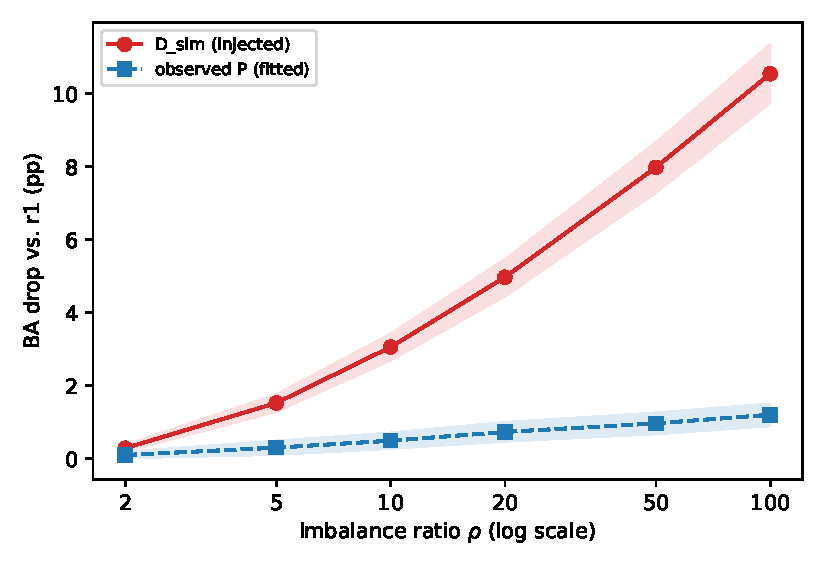
\includegraphics[width=0.49\textwidth]{onset_curve_tcga_ut.pdf}
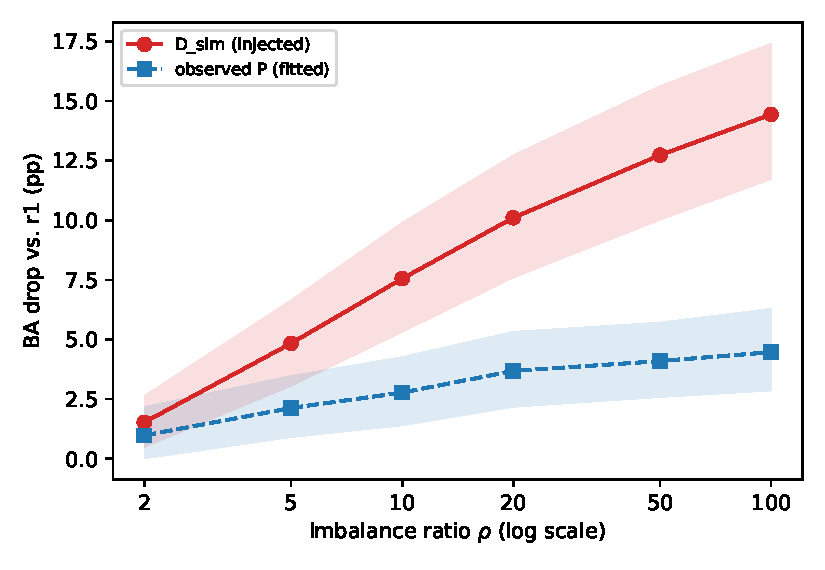
\includegraphics[width=0.49\textwidth]{onset_curve_bracs.pdf}
\caption{The simulated damage $D_{\mathrm{sim}}(\rho)$ (red, injected into the frozen balanced decision surface) against the already-fitted prior-only damage P$(\rho)$ (blue, from a genuine reweighted refit), on TCGA-UT (left) and BRACS (right). Points are pooled over three splits and ten draws per split; bands are 95 percent bootstrap intervals. The two curves track each other only at the smallest ratio.}
\label{fig:onset}
\end{figure}

\subsection{H3: a class-count control does not bring BRACS back onto the trend}
\label{sec:h3-result}
Restricting TCGA-UT's balanced model to 500 random seven-class subsets of its 30 classes, and injecting a synthetic $\rho=100$ profile with a random class-to-rank assignment within each subset, produces a strong negative relationship between how hard a subset already is and how much the injection damages it: Spearman correlations of $-0.53$ ($p<10^{-37}$) between a subset's own balanced accuracy and its simulated damage, and $-0.55$ ($p<10^{-39}$) between its median margin and its simulated damage. Both are shown in Figure~\ref{fig:subsets}. A subset built by greedily growing the group of seven classes with the largest pairwise confusion rate lands at a balanced accuracy of 58.5 percent, a median margin of 0.60 nats, and a simulated damage of 9.15 points, below the random subsets' own minimum balanced accuracy of 67.4 percent and consistent with the same trend.

BRACS's own balanced accuracy under its balanced arm, 39.6 percent, and its own median margin, 0.27 nats, both fall outside the entire range covered by the 500 random subsets, whose balanced accuracy spans 67.4 to 97.4 percent and whose median margin spans 0.96 to 5.93 nats, and outside the range reached by the single most-confused engineered subset as well. Restricting TCGA-UT to seven classes, even a deliberately hard seven, does not reproduce a task as separability-poor as BRACS's native seven. A narrower class count on its own is therefore not sufficient to place BRACS back on the trend line these subsets trace; whatever makes BRACS's classes harder to tell apart under balanced training is not simply a consequence of having fewer of them.

\begin{figure}[htbp]
\centering
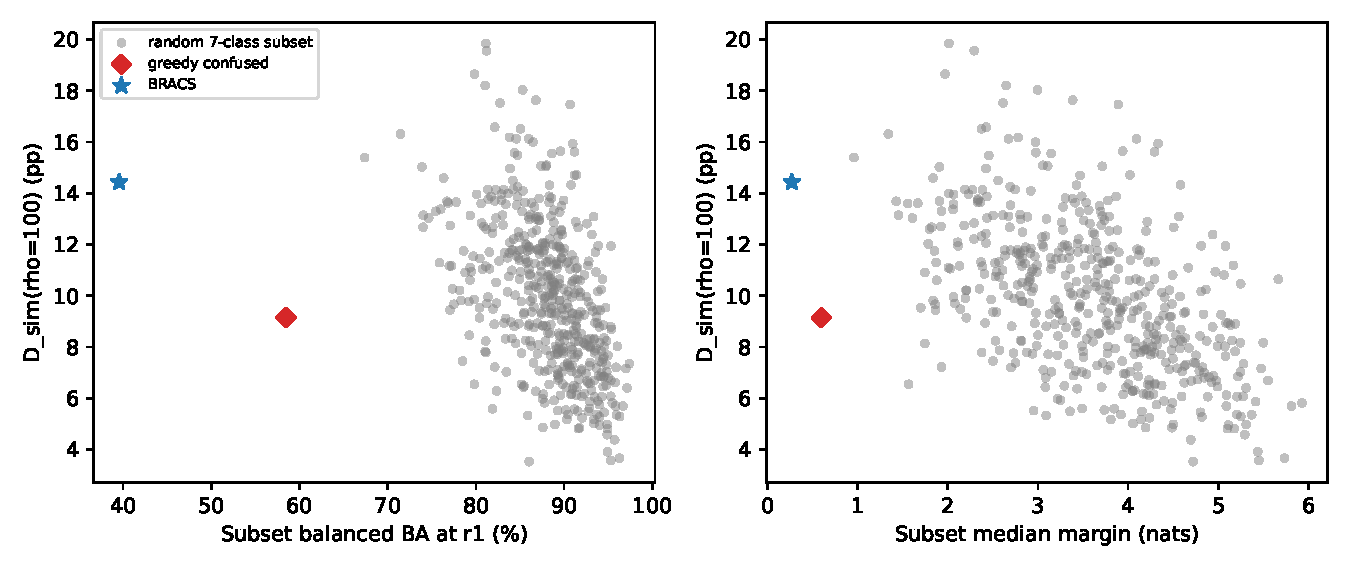
\includegraphics[width=\textwidth]{subset_scatter_tcga_ut.pdf}
\caption{Simulated $\rho=100$ damage against a seven-class subset's own balanced accuracy (left) and median margin (right), for 500 random seven-class subsets of TCGA-UT's 30 classes (grey), the single subset built from the seven most pairwise-confused classes (red diamond), and BRACS's own balanced arm (blue star). BRACS falls outside the range every TCGA-UT subset covers on both axes.}
\label{fig:subsets}
\end{figure}

\noindent Figure~\ref{fig:margins} shows why a shared $\rho=100$ profile produces such different damage on the two full datasets: BRACS's test-patch margin distribution sits far closer to zero than TCGA-UT's, so a much larger share of its patches fall within the log-count gap the injected prior introduces at any of the three marked ratios.

\begin{figure}[htbp]
\centering
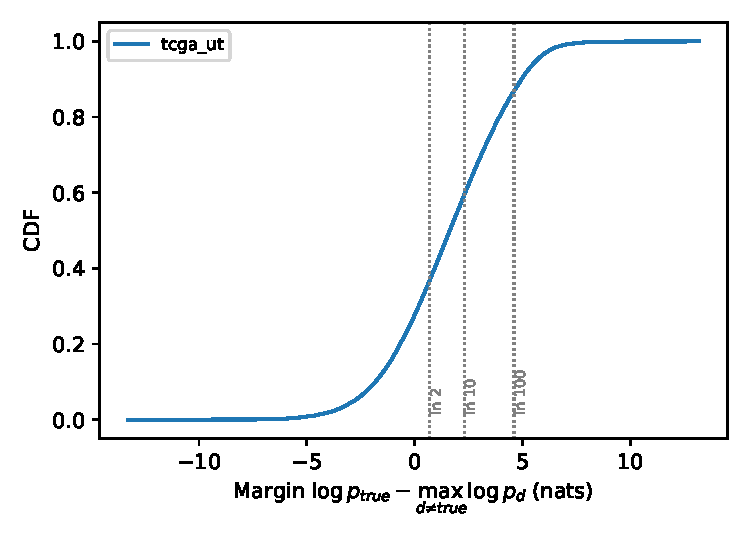
\includegraphics[width=0.49\textwidth]{margin_cdf_tcga_ut.pdf}
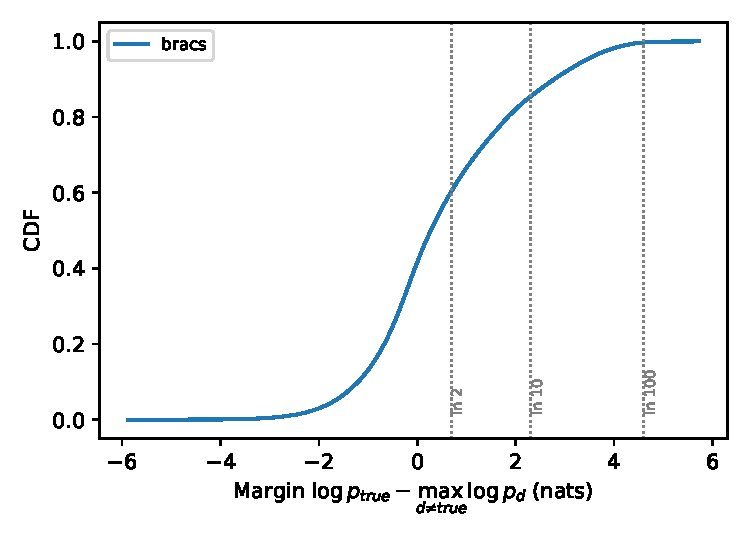
\includegraphics[width=0.49\textwidth]{margin_cdf_bracs.pdf}
\caption{Cumulative distribution of the balanced arm's test-patch margin, $\log p_{\mathrm{true}} - \max_{d\neq\mathrm{true}} \log p_d$, on TCGA-UT (left, median 1.63 nats) and BRACS (right, median 0.27 nats). Vertical lines mark $\ln\rho$ for $\rho\in\{2,10,100\}$: the share of patches with a smaller margin than a given line is the share directly exposed to a prior shift of that size.}
\label{fig:margins}
\end{figure}

The validation-temperature-scaled sensitivity variant lowers the simulated damage but does not close the gate. Injecting the same prior into calibrated rather than raw probabilities gives $D_{\mathrm{sim,TS}}(100)=7.74$ points on TCGA-UT and $9.01$ points on BRACS, 2.81 and 5.42 points below the raw-probability values respectively; both remain well outside their dataset's fitted P100 interval. Calibration narrows the damage, consistent with temperature scaling spreading probability mass away from the single most likely class and so softening how much a fixed log-prior shift can move an argmax, but it does not narrow it enough to make the injection a valid stand-in for a genuine refit.

\section{Discussion}
\label{sec:discussion}
Injecting a fitted dataset's own realized class prior into its balanced model's stored decisions was meant to give a zero-fit stand-in for the fitted prior-only damage, one that keeps the margins, the direction, and the class count a linear confusion score discards. It does keep all three, and its failure is informative about exactly which of them dominates: Section~\ref{sec:h2-result} shows the simulated and fitted curves agreeing only where the injected shift is small enough that few decisions move, and Section~\ref{sec:h3-result} shows the simulated damage tracking a subset's own margin closely within one dataset. What the simulation does not do is reproduce the size of a genuine refit's damage once the shift is large. A reweighted refit redistributes an entire decision surface to accommodate a new prior; the injection used here moves every decision independently against a surface that was never asked to accommodate one, so wherever a patch's margin is smaller than the injected log-prior gap, the prediction flips regardless of whether a refit would have found a way to keep it. This is the same margin-sensitivity that motivated using simulation over a linear score in the first place, and it turns out to be strong enough that the simulation overshoots a genuine refit's damage by a wide margin once $\rho$ moves past the smallest ratio tested.

The size of that overshoot is itself dataset-dependent in a way median margin alone does not explain: TCGA-UT's balanced arm has the larger median margin of the two datasets, 1.63 against BRACS's 0.27 nats, yet TCGA-UT's simulation overshoots its own fitted damage by roughly seven times against BRACS's roughly three times. A median summarizes the typical patch, while the injected damage is set by whichever patches sit closest to the decision boundary in either direction; with thirty classes, TCGA-UT's balanced model has many more pairwise boundaries than BRACS's seven-class model does, and it is plausible that this gives more opportunities for some pair's margin to be smaller than the injected gap even when the typical margin is comparatively large. This report does not test that account and does not extend it into a mechanism claim; it is offered only to keep the size of the gate's failure from reading as a single fixed multiplier that a future report could simply divide out.

What the class-count control in Section~\ref{sec:h3-result} does show, without needing the gate to pass, is that BRACS's balanced arm is harder, in both accuracy and margin terms, than any seven-class subset carved from TCGA-UT, including the one deliberately built to maximize pairwise confusion. If the 3.27-point fitted gap between the two datasets' prior-only damage has a cause that generalizes past class count, it is a property of how BRACS's seven classes overlap under balanced training that a same-sized slice of TCGA-UT's thirty classes does not share, not an artifact of TCGA-UT's larger label set diluting its own damage. That leaves the fitted gap's cause open. The prior channel investigated here explains at most part of it, and the support channel, thin tail patch counts rather than a shifted prior, carries a comparable or larger share of BRACS's total $\rho=100$ damage in the companion prior-versus-support study \citep{queisler2026causeBracs} and remains untested for why it costs more on BRACS than on TCGA-UT. A companion patient-shortage study finds that most of the benefit of additional patients on a related task comes from a class-centre error rather than from added support directly \citep{queisler2026centreError}; whether an analogous centre-error account explains the support channel's dataset gap is the natural next candidate and is left open here.

\section{Limitations}
\label{sec:limitations}
Gate G is a necessary check on one proxy's absolute validity, not a diagnosis of what is wrong with it; failing it rules the proxy out for a mechanism claim without identifying which of the reasons discussed above is the operative one. H1's numerical agreement with the fitted gap is reported for the record and is explicitly not evidence for the prior-channel account, since it survives only as a difference of two independently wrong quantities. H3's restricted-softmax subsets are not retrained seven-class models: renormalizing an already-fit thirty-class softmax over seven columns changes what probability mass is available to redistribute in a way an actual seven-class refit would not, so the subset scores in Figure~\ref{fig:subsets} should be read as a screen for whether class count alone can explain BRACS's position, not as a measurement of what a seven-class TCGA-UT model would show. The greedy confused-class subset uses a single, un-bootstrapped pooled confusion matrix from the balanced arm and is one specific construction among many that could grow a hard subset; a different growth rule could plausibly find a harder one. All results are conditional on the same design as the prior-versus-support studies: frozen Virchow2 features, multinomial logistic regression, the same three splits and ten draws per split, $G=20$ patients per class on TCGA-UT and $G=10$ on BRACS, and the class-rank permutation scheme of the prevalence curves \citep{queisler2026prevalenceTcga, queisler2026prevalenceBracs, queisler2026causeTcga, queisler2026causeBracs}.
